%% CILP manuscript — Journal of Big Data Methodology draft
\documentclass[11pt,a4paper]{article}

\usepackage[margin=2.5cm]{geometry}
\usepackage{times}
\usepackage{mathtools,amssymb,bm}
\usepackage{booktabs,multirow,longtable,tabularx,array}
\usepackage{graphicx}
\usepackage{xcolor}
\usepackage[hidelinks]{hyperref}
\usepackage{natbib}
\usepackage{setspace}
\usepackage{enumitem}
\usepackage{caption}
\usepackage{tikz}
\usetikzlibrary{arrows.meta,positioning,calc}
\usepackage{fancyhdr}
\usepackage{titlesec}
\usepackage{microtype}
\usepackage{placeins}
\usepackage{lineno}

\doublespacing
\linenumbers
\setlength{\headheight}{14pt}
\setlength{\parskip}{0em}
\setlength{\parindent}{1.1em}

\titleformat{\section}{\large\bfseries}{\thesection}{0.55em}{}
\titleformat{\subsection}{\normalsize\bfseries}{\thesubsection}{0.45em}{}

\pagestyle{fancy}
\fancyhf{}
\fancyhead[L]{\textit{CILP --- Journal of Big Data Methodology draft}}
\fancyhead[R]{\thepage}
\renewcommand{\headrulewidth}{0.3pt}

\newcommand{\cilp}{CILP}
\newcommand{\ilp}{ILP-GCN}

\begin{document}

\begin{center}
{\LARGE\bfseries Learning which edges to remove under a budget:\\
Counterfactual inverse link prediction for utility-preserving\\
social-network sparsification\par}
\vspace{1.0em}
% Authors and affiliations: finalize before submission.
% Corresponding author: finalize before submission.
{\large\textit{Journal of Big Data --- Methodology article draft}\par}
\vspace{0.8em}
\end{center}

\begin{abstract}
Edge-rich attributed social networks inflate storage and message-passing cost in graph neural networks, motivating utility-preserving sparsification under an exact edge-removal budget.
We present Counterfactual Inverse Link Prediction (CILP), which extends inverse link prediction from cheminformatics similarity graphs to attributed social networks through composite counterfactual supervision.
CILP trains an edge scorer with a multi-criteria teacher that combines deletion-induced effects (task loss, connectivity, representation shift, and group impact) with structural proxies (community-boundary and degree-based spectral terms), and removes low-importance edges by unconstrained ranking under a matched budget.
On LastFM Asia, Facebook Page-Page, and GitHub Developers (ten paired seeds; removal rates $0.1$--$0.9$), CILP improves sparsity--Macro-F1 AUC over an architecturally matched task-only teacher by $+0.0265$, $+0.0142$, and $+0.0033$, respectively, and improves all four paired evaluation metrics over Task-only on each dataset after within-dataset Holm correction.
CILP remains competitive with ILP-GCN and PTDNet, but does not universally lead predictive AUC.
CILP training, which includes teacher construction and scorer fitting, is substantially more expensive than the lighter baselines.
The supported contribution is multi-criteria counterfactual supervision under matched budgets, not universal predictive or structural superiority.
\end{abstract}

\noindent\textbf{Keywords:}
Inverse link prediction; graph sparsification; social networks; graph neural networks; counterfactual learning; edge importance; multi-criteria learning

\section{Introduction}
\label{sec:intro}

Attributed social networks used for recommendation, influence analysis, and community detection are large and edge-rich: edge counts are substantial even when classical density $2|E|/(|V|(|V|-1))$ is small.
Message-passing graph neural networks (GNNs) scale with the number of edges: each training epoch aggregates neighbourhood messages, stores activations, and pays memory proportional to edge volume~\citep{kipf2017semi,rong2020dropedge}.
Reducing edges under an exact removal budget therefore addresses a concrete big-data systems constraint---storage, communication, and wall-clock training cost---provided downstream predictive utility and key connectivity properties are not destroyed~\citep{zheng2020neuralsparse,luo2021ptdnet,spielman2011graph}.

This paper sits at the intersection of link prediction, inverse link prediction, and graph sparsification.
Link prediction estimates missing or future edges~\citep{liben2007link,martinez2016survey}.
Inverse link prediction reverses that direction: it ranks \emph{existing} edges by deletion harm under a budget, aiming to preserve utility rather than to invent new links~\citep{bangian2025ilp}.
Structure-preserving and spectral sparsification motivate edge removal while retaining important graph properties~\citep{lindner2015structure,hamann2016structure,chen2024demystifying,feng2016spectral,spielman2011graph}; learned GNN sparsifiers further show that pruning can be task-aware~\citep{zheng2020neuralsparse,luo2021ptdnet,li2020sgcn}.
Inverse link prediction with graph convolutional networks was introduced for cheminformatics similarity graphs by Bangian Tabrizi, Jalali and Houshmand~\citep{bangian2025ilp}; we refer to that parent method as the original ILP-GCN method, and thereafter as ILP-GCN.
Counterfactual Inverse Link Prediction (CILP) extends ILP-GCN to attributed social networks through composite counterfactual supervision: a multi-criteria teacher labels deletion importance, a GCN scorer learns the ranking, and edges are removed under equal exact budgets.

Edge deletion is established in counterfactual GNN explanation~\citep{lucic2022cfgnn,pradoromero2022gretel,funke2022zorro,mastropietro2022edgeshaper}, and learning edge importance for pruning is likewise established~\citep{zheng2020neuralsparse,luo2021ptdnet,rong2020dropedge,li2020sgcn}.
CILP does not claim to invent edge deletion, edge scoring, graph sparsification, or counterfactual GNN explanation.
Its methodological element is a composite multi-criteria teacher that combines deletion-induced effects with structural proxies, learned by a GCN scorer and applied under matched exact budgets.
Counterfactual probing is expensive on CPU, but for a fixed graph and seed the teacher/scorer are built once and then reused to produce rankings at every removal budget $r\in\{0.1,\ldots,0.9\}$.
This amortizes construction across budgets for that seed; it does not by itself demonstrate amortization across repeated independent downstream training runs.
We compare CILP with an architecturally matched task-only teacher---the central controlled comparison---and with ILP-GCN, PTDNet, NeuralSparse, Random, and a Resistance proxy.
The evaluation covers three attributed social networks (LastFM Asia, Facebook Page-Page, and GitHub Developers) with ten paired seeds and removal rates $0.1$--$0.9$.
Methods are judged under equal removal budgets; the main claim is a consistent multi-criteria-supervision benefit relative to the matched task-only teacher, not overall leadership over every baseline.
We do not claim large-scale GPU throughput: the reported implementation is CPU-bound, and CILP training (teacher construction plus scorer fitting) remains substantially more expensive than lighter baselines.

The remainder of the paper follows a Methodology organization: related work, the proposed CILP method, experimental setup, results, discussion, and conclusions.

\section{Related work}
\label{sec:related}

This study sits at the intersection of link prediction, inverse link prediction, and graph sparsification.
Classical link prediction asks which missing or future edges are likely to form~\citep{liben2007link,martinez2016survey}.
Inverse link prediction reverses that question: given an exact removal budget, which \emph{existing} edges should be deleted so that predictive utility and selected structural properties are preserved~\citep{bangian2025ilp}.
Graph sparsification provides the structural motivation for edge removal~\citep{lindner2015structure,hamann2016structure,chen2024demystifying,feng2016spectral,spielman2011graph}, while learned GNN sparsifiers show that pruning can be made task-aware rather than purely structural~\citep{luo2021ptdnet,zheng2020neuralsparse,li2020sgcn,li2022gcnsparsify}.
Utility-aware evaluation in link recommendation further argues that accuracy alone is an incomplete performance lens~\citep{sanzcruzado2018novelty,mara2022evalne,li2017utility}.

\subsection{Link prediction}
The link-prediction problem for social networks estimates missing or future edges from network structure~\citep{liben2007link}.
Surveys cover neighbourhood heuristics, path-based scores, probabilistic models, and embedding-based predictors~\citep{martinez2016survey}.
That literature is concerned with \emph{adding} or recovering edges.
CILP uses the same social-network setting but asks which edges to \emph{remove} under a budgeted sparsification objective.

\subsection{Inverse link prediction and budgeted edge removal}
ILP-GCN ranks existing edges for knowledge-preserving sparsification of cheminformatics similarity graphs~\citep{bangian2025ilp}.
CILP retains the inverse-link-prediction question but changes the edge target, graph domain, selection rule, and evaluation protocol (Table~\ref{tab:advance}): a composite multi-criteria counterfactual teacher supervises a GCN scorer on attributed social networks under matched exact budgets.
The present work is therefore an extension of inverse link prediction into utility-preserving social-network sparsification, not a new link-prediction accuracy method.

\subsection{Structure-preserving and spectral sparsification}
Structure-preserving sparsifiers rate edges by importance and filter globally or locally to retain connectivity, distances, communities, and centrality patterns in social networks~\citep{lindner2015structure,hamann2016structure}.
Comparative studies show that no single sparsifier preserves all graph properties equally well; suitability depends on the downstream metric family~\citep{chen2024demystifying}.
Spectral sparsification seeks sparse subgraphs whose Laplacians approximate the original spectrum, including effective-resistance sampling~\citep{spielman2011graph} and nearly-linear-time constructions based on spectral perturbation analysis~\citep{feng2016spectral}.
CILP borrows structural proxies (community and degree-based spectral terms) as teacher components, but ranks edges for budgeted GNN utility rather than classical cut or Laplacian approximation alone.

\subsection{Learned sparsification with graph neural networks}
DropEdge randomly drops edges during training~\citep{rong2020dropedge}.
NeuralSparse and PTDNet learn to remove task-irrelevant edges for robust representation learning~\citep{zheng2020neuralsparse,luo2021ptdnet}.
SGCN and related GCN sparsifiers prune edges by optimization so that node-classification performance is retained on a sparser graph~\citep{li2020sgcn,li2022gcnsparsify}.
Learning to prune is therefore established.
CILP's distinct element is inverse-link-prediction-style scoring supervised by a composite counterfactual teacher under equal social-network budgets, with an architecturally matched task-only ablation as the primary controlled comparison.

\subsection{Utility-aware evaluation beyond accuracy}
Utility-based link recommendation incorporates value and cost beyond linkage likelihood~\citep{li2017utility}.
Structural novelty and diversity metrics likewise argue that link-centric evaluation should consider network effects beyond predictive accuracy~\citep{sanzcruzado2018novelty}.
Evaluation frameworks such as EvalNE systematize reproducible link-prediction assessment for network embeddings~\citep{mara2022evalne}.
We adopt a related stance for sparsification: Macro-F1 under exact budgets is reported jointly with connectivity, bridge retention, and minority-degree retention, rather than accuracy alone.

\subsection{Counterfactual GNN explanation}
Graph counterfactual explanation methods intervene on graphs---often by deleting or editing edges---to change a GNN decision while remaining sparse or valid~\citep{lucic2022cfgnn,pradoromero2022gretel,funke2022zorro,mastropietro2022edgeshaper}.
GRETEL formalizes evaluation practice for this family~\citep{pradoromero2022gretel}; Zorro emphasizes fidelity and stability~\citep{funke2022zorro}; EdgeSHAPer attributes edge contributions~\citep{mastropietro2022edgeshaper}.
These methods target local explanation or recourse.
CILP instead uses deletion probes and structural proxies to supervise global budgeted sparsification, which is a different objective from flipping an individual prediction with few edits~\citep{agarwal2023evaluating}.

\section{Proposed CILP methodology}
\label{sec:methods}

\subsection{Problem formulation}
Given an attributed undirected graph $G=(V,E,X,Y)$ and edge-removal rate $r\in[0,1]$, return a sparsified edge set $E_r\subseteq E$ with
\[
|E_r|=(1-r)|E|
\]
(all nodes retained). Write $G_r=(V,E_r,X,Y)$ for the sparsified graph.
Downstream GCN Macro-F1 is the primary utility metric~\citep{kipf2017semi}.

\subsection{Advance relative to ILP-GCN}
Table~\ref{tab:advance} summarizes the methodological differences.
The social-network domain alone is not presented as novelty; the new element under study is composite counterfactual supervision with a matched task-only control under exact budgets.

\begin{table}[t]
\centering
\caption{\textbf{Methodological advance of CILP relative to ILP-GCN.}}
\label{tab:advance}
\scriptsize
\begin{tabular}{@{}p{2.2cm}p{5.3cm}p{5.8cm}@{}}
\toprule
Aspect & ILP-GCN~\citep{bangian2025ilp} & CILP \\
\midrule
Graph domain & Cheminformatics similarity graph & Attributed social graph \\
Edge target & Inverted link probability & Composite multi-criteria teacher \\
Criteria & Link score (and domain priors in the parent setting) & Task loss, connectivity, community-boundary proxy, degree-based spectral proxy, representation shift, group impact \\
Selection & Threshold / modularity-oriented sparsification in the parent paper & Exact-budget ranking by predicted importance $\mu_e$ \\
Uncertainty & Not used for ranking & Heteroscedastic $\sigma_e$ estimated but unused for ranking in reported runs \\
Evaluation & Domain-graph sparsification & Multi-seed social-network utility and structure under matched budgets \\
Main control & Random / classical baselines & Architecturally matched task-only teacher \\
\bottomrule
\end{tabular}
\end{table}

\subsection{Composite multi-criteria teacher}
CILP uses a composite multi-criteria teacher that combines deletion-induced effects with structural proxies (Fig.~\ref{fig:framework}).
Sample $n$ edges, delete each edge as required, and compute six normalized deletion-importance criteria (Supplementary Information~S5--S6):
\begin{itemize}[leftmargin=1.4em]
\item \textbf{Deletion-induced:} task loss, connectivity change, representation shift, group impact;
\item \textbf{Structural proxies:} community-boundary proxy, degree-based spectral proxy.
\end{itemize}
\[
y_e^{\mathrm{cf}}=\mathrm{minmax}\Big(\sum_k\beta_k\,\mathrm{minmax}(\Delta_k(e))\Big),
\]
with fixed weights $\beta=(1.0,0.5,1.0,0.3,0.5,0.5)$ for
(task, community-boundary proxy, connectivity, degree-based spectral proxy, representation, group),
identical across datasets and not development-tuned.
This is weighted-sum scalarization, not Pareto optimization.
The matched task-only teacher uses $y=\mathrm{minmax}(\Delta_{\mathrm{task}})$ with the same encoder and concatenation fusion.

\begin{figure}[t]
\centering
\resizebox{\textwidth}{!}{% Figure 1 — CILP framework
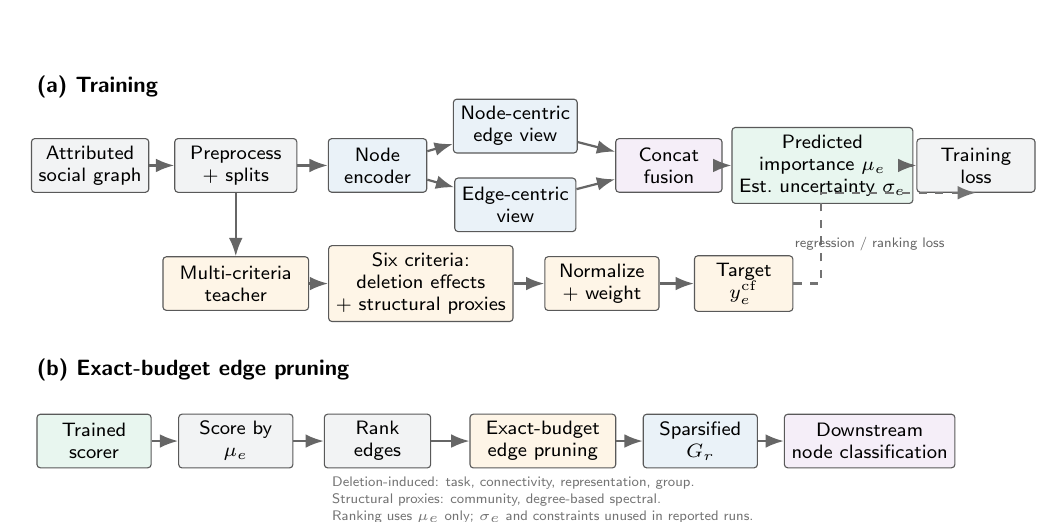
\begin{tikzpicture}[
  font=\sffamily\scriptsize,
  >=Latex,
  box/.style={draw=black!65, rounded corners=1.2pt, align=center, inner sep=2.6pt, fill=#1, minimum height=0.68cm},
  arr/.style={->, thick, black!60},
  dasharr/.style={->, thick, dashed, black!55},
  plab/.style={font=\sffamily\footnotesize\bfseries, anchor=west},
]
\definecolor{cA}{HTML}{EAF2F8}
\definecolor{cB}{HTML}{E8F6EF}
\definecolor{cC}{HTML}{FEF5E7}
\definecolor{cD}{HTML}{F5EEF8}
\definecolor{cE}{HTML}{F2F3F4}

\node[plab] at (-0.15,3.35) {(a) Training};
\node[box=cE, minimum width=1.45cm] (g) at (0.65,2.35) {Attributed\\social graph};
\node[box=cE, minimum width=1.55cm] (pp) at (2.5,2.35) {Preprocess\\+ splits};
\node[box=cA, minimum width=1.25cm] (enc) at (4.3,2.35) {Node\\encoder};
\node[box=cA, minimum width=1.45cm] (nv) at (6.05,2.85) {Node-centric\\edge view};
\node[box=cA, minimum width=1.45cm] (ev) at (6.05,1.85) {Edge-centric\\view};
\node[box=cD, minimum width=1.35cm] (fus) at (8.0,2.35) {Concat\\fusion};
\node[box=cB, minimum width=1.7cm] (dec) at (9.95,2.35) {Predicted\\importance $\mu_e$\\Est.\ uncertainty $\sigma_e$};
\node[box=cE, minimum width=1.5cm] (loss) at (11.9,2.35) {Training\\loss};

\draw[arr] (g)--(pp); \draw[arr] (pp)--(enc);
\draw[arr] (enc)--(nv); \draw[arr] (enc)--(ev);
\draw[arr] (nv)--(fus); \draw[arr] (ev)--(fus);
\draw[arr] (fus)--(dec); \draw[arr] (dec)--(loss);

\node[box=cC, minimum width=1.85cm] (samp) at (2.5,0.85) {Multi-criteria\\teacher};
\node[box=cC, minimum width=2.15cm] (del) at (4.85,0.85) {Six criteria:\\deletion effects\\+ structural proxies};
\node[box=cC, minimum width=1.45cm] (agg) at (7.15,0.85) {Normalize\\+ weight};
\node[box=cC, minimum width=1.25cm] (ycf) at (8.95,0.85) {Target\\$y^{\mathrm{cf}}_e$};
\draw[arr] (pp)--(samp); \draw[arr] (samp)--(del); \draw[arr] (del)--(agg); \draw[arr] (agg)--(ycf);
\draw[dasharr] (ycf.east) -- ++(0.35,0) |- (loss.south);
\node[font=\sffamily\tiny, text=black!60] at (10.55,1.35) {regression / ranking loss};

\node[plab] at (-0.15,-0.25) {(b) Exact-budget edge pruning};
\node[box=cB, minimum width=1.45cm] (sc) at (0.7,-1.15) {Trained\\scorer};
\node[box=cE, minimum width=1.45cm] (score) at (2.5,-1.15) {Score by\\$\mu_e$};
\node[box=cE, minimum width=1.35cm] (rank) at (4.3,-1.15) {Rank\\edges};
\node[box=cC, minimum width=1.85cm] (pr) at (6.4,-1.15) {Exact-budget\\edge pruning};
\node[box=cA, minimum width=1.45cm] (sp) at (8.4,-1.15) {Sparsified\\$G_r$};
\node[box=cD, minimum width=2.0cm] (evl) at (10.55,-1.15) {Downstream\\node classification};
\draw[arr] (sc)--(score); \draw[arr] (score)--(rank); \draw[arr] (rank)--(pr);
\draw[arr] (pr)--(sp); \draw[arr] (sp)--(evl);
\node[font=\sffamily\tiny, text=black!55, align=left] at (6.4,-1.9) {Deletion-induced: task, connectivity, representation, group.\\
Structural proxies: community, degree-based spectral.\\
Ranking uses $\mu_e$ only; $\sigma_e$ and constraints unused in reported runs.};
\end{tikzpicture}
}
\caption{\textbf{Schematic of Counterfactual Inverse Link Prediction (CILP).}
\textbf{a}~Forward scoring path with a parallel multi-criteria teacher providing targets $y^{\mathrm{cf}}_e$.
Four criteria are deletion-induced effects; community-boundary and degree-based spectral terms are structural proxies.
\textbf{b}~Exact-budget edge pruning by predicted importance $\mu_e$ and downstream node classification.
Reported runs rank by $\mu_e$ only; $\sigma_e$ and optional constraints are unused.}
\label{fig:framework}
\end{figure}

\subsection{Edge scorer and fusion}
A 2-layer GCN encoder (hidden dimension $64$, dropout $0.4$) produces node embeddings.
Node-centric and edge-centric edge representations are combined by concatenation in the core comparison; gated and cross-attention fusions are ablations only.
A heteroscedastic decoder outputs $(\mu_e,\log\sigma_e^2)$.
Training minimizes a weighted sum of classification cross-entropy, Gaussian NLL, and ranking hinge loss (Supplementary Information~S9, S13).

\subsection{Exact-budget pruning}
Reported runs keep the top $(1-r)|E|$ edges by descending $\mu_e$, with
$n_{\mathrm{keep}}=|E|-\mathrm{round}(r|E|)$.
Estimated uncertainty $\sigma_e$ is not used for ranking.
Optional constraint-aware pruning exists in code but is disabled in the multi-seed comparison.

\section{Experimental setup}
\label{sec:setup}

\subsection{Datasets and preprocessing}
LastFM Asia and GitHub Developers are obtained from SNAP archives; Facebook Page-Page from MUSAE~\citep{rozemberczki2021multi}.
Edges are symmetrized; self-loops and duplicate undirected edges are removed; bag-of-words indices are expanded to multi-hot features.
Table~\ref{tab:datasets} summarizes sizes.
Although classical densities are low (${\sim}4{\times}10^{-4}$--$1{\times}10^{-3}$), edge volumes are large enough to contribute substantially to GNN message-passing cost.
All three datasets are included in the completed multi-seed evaluation.

\begin{table}[t]
\centering
\caption{\textbf{Dataset characteristics.}}
\label{tab:datasets}
\begin{tabular}{@{}lrrrr@{}}
\toprule
Dataset & Nodes & Edges & Classes & Feature dim. \\
\midrule
LastFM Asia & 7\,624 & 27\,806 & 18 & 7\,842 \\
Facebook Page-Page & 22\,470 & 170\,823 & 4 & 4\,714 \\
GitHub Developers & 37\,700 & 289\,003 & 2 & ${\sim}$4\,005 \\
\bottomrule
\end{tabular}
\end{table}

\subsection{Splits and leakage control}
Seeds $0$--$9$ use stratified $60/20/20$ node masks shared by every method on each dataset.
We refer to the middle partition as a \emph{development} set rather than an independent validation set: it is used both in teacher $\Delta_{\mathrm{task}}$ construction (cross-entropy on train$\cup$development) and, for Facebook, in teacher-size selection (development Macro-F1 at $50\%$ removal).
Test labels are used only for final evaluation after the configuration is fixed (Supplementary Information~S4).
This is not test leakage, but the development partition is not a fully isolated model-selection hold-out.
A stricter protocol that builds teacher targets from training labels alone is left as a recommended refinement.
Facebook teacher size $n{=}120$ was selected by development Macro-F1 at $50\%$ removal; LastFM uses $n{=}50$; GitHub uses $n{=}40$.
GitHub teacher/scorer/downstream/ILP epoch budgets are $15/15/35/15$; criterion weights $\beta$ are fixed and identical across datasets.

\subsection{Baselines and matched control}
Comparators: Random, ILP-GCN~\citep{bangian2025ilp}, Task-only (matched ablation), NeuralSparse, PTDNet~\citep{zheng2020neuralsparse,luo2021ptdnet}, and Resistance proxy~\citep{spielman2011graph}.
The Resistance proxy implements an effective-resistance-inspired ranking; it is not an independent reproduction of DSpar.
Duplicate records from the same resistance-based implementation were removed before aggregation.

\subsection{Evaluation metrics and statistics}
We report Macro-F1, sparsity--Macro-F1 AUC over removal rates $0.1$--$0.9$, giant-component ratio, bridge retention, minority-degree retention, surrogate agreement, and wall-clock training time.
Paired Wilcoxon signed-rank tests are used for hypothesis testing; paired $t$-distributions supply confidence intervals for mean differences (intervals are not accompanied by paired $t$ $p$-values in the tables).
Wilcoxon tests are two-sided, applied to paired seed-wise differences with SciPy defaults (\texttt{zero\_method='wilcox'}, \texttt{correction=False}, \texttt{method='auto'}; for $n{=}10$ this yields an exact enumeration when no ties force an approximation).
Zero differences are discarded under \texttt{wilcox}; remaining ties among nonzero ranks follow SciPy's standard mid-rank handling.
Effect sizes use paired $d_z$; intervals use $t_{0.975,n-1}\mathrm{SEM}$~\citep{wilcoxon1945individual,holm1979simple,cohen1988statistical}.
Two Holm families are distinguished:
(i)~within each dataset, the four CILP-versus-Task-only metrics (AUC; giant-component, bridge, and minority-degree retention at $50\%$);
(ii)~within each dataset, CILP-versus-baseline AUC contrasts across methods.
Adjusted $p$-values are therefore not interchangeable across families.
Multi-criteria supervision is treated as supported on a dataset when at least two of the four seed-aligned metrics improve under identical fusion after Holm adjustment in family~(i); across-dataset support requires that criterion on at least two datasets (Supplementary Information~S21).
The analysis rule was fixed before completion and integration of the GitHub grid; we do not claim timestamped preregistration outside the repository freeze record.

\subsection{Computational protocol}
All reported multi-seed runs used CPU execution in PyTorch Geometric; MPS is disabled in the device helper.
Full hyperparameter and software details appear in Supplementary Information~S13 and~S27.
Reported CILP and Task-only \texttt{train\_seconds} include teacher construction and scorer fitting; these components were not logged separately, so we do not attribute dominance to teacher construction alone.
The full GitHub grid (seven methods, seeds $0$--$9$, budgets $0.1$--$0.9$) completed with no method failures; orchestration wall-clock was approximately $6.19$\,h.
Per-method training times are reported from the authoritative runtime table and are distinct from that orchestration total.

\section{Results}
\label{sec:results}

Completed multi-seed results cover LastFM Asia, Facebook Page-Page, and GitHub Developers ($n{=}10$ seeds; budgets $0.1$--$0.9$; $1{,}890$ authoritative rows).

\subsection{Main multi-seed sparsification results}
Figure~\ref{fig:curves} and Table~\ref{tab:main} report Macro-F1 versus edge-removal rate ($n{=}10$ seeds on all three datasets).

\begin{figure}[t]
\centering
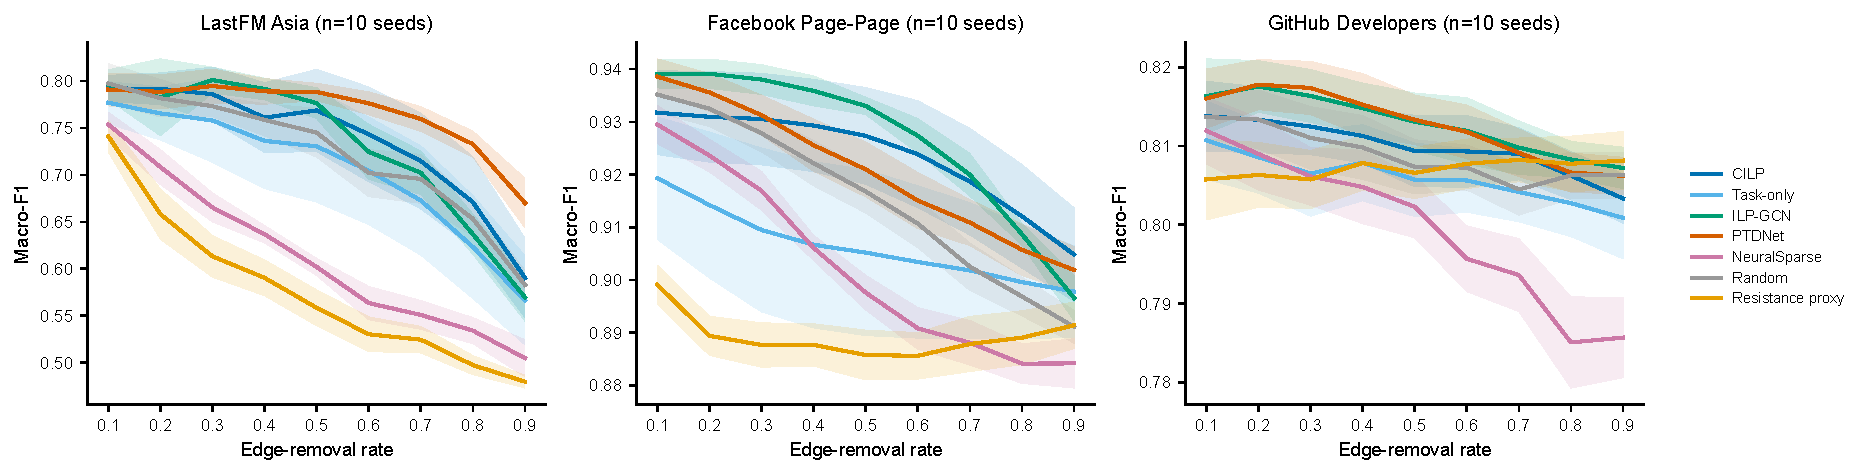
\includegraphics[width=\linewidth]{figures/fig2_sparsity_curves.pdf}
\caption{\textbf{Sparsity--Macro-F1 curves.}
Mean Macro-F1 versus edge-removal rate; bands are $95\%$ $t$-intervals (mean $\pm t_{0.975,n-1}\mathrm{SEM}$) with $n{=}10$ seeds.
Panels use dataset-specific $y$-axis ranges.
Curves begin at $10\%$ removal; a full-graph ($0\%$) reference is not included in the present grid.
Legend order: CILP, Task-only, ILP-GCN, PTDNet, NeuralSparse, Random, Resistance proxy.}
\label{fig:curves}
\end{figure}

\begin{table}[t]
\centering
\caption{\textbf{Main predictive results} (mean$\pm$s.d., $n{=}10$ seeds $0$--$9$).
AUC: trapezoidal sparsity--Macro-F1 area over edge-removal rates $0.1$--$0.9$.
\textbf{Bold}: best mean in each column within a dataset; \underline{underline}: second-best (ties shared).
Visual ranking does not imply statistical significance.}
\label{tab:main}
\scriptsize
\begin{tabular}{@{}llcccc@{}}
\toprule
Dataset & Method & 30\% & 50\% & 70\% & AUC \\
\midrule
\multirow{7}{*}{LastFM}
& PTDNet & $\underline{0.795}{\pm}0.025$ & $\textbf{0.788}{\pm}0.013$ & $\textbf{0.760}{\pm}0.018$ & $\textbf{0.616}{\pm}0.011$ \\
& CILP & $0.786{\pm}0.040$ & $0.769{\pm}0.061$ & $\underline{0.715}{\pm}0.071$ & $\underline{0.593}{\pm}0.038$ \\
& ILP-GCN & $\textbf{0.801}{\pm}0.019$ & $\underline{0.776}{\pm}0.023$ & $0.702{\pm}0.032$ & $0.590{\pm}0.017$ \\
& Random & $0.773{\pm}0.016$ & $0.745{\pm}0.036$ & $0.696{\pm}0.036$ & $0.580{\pm}0.018$ \\
& Task-only & $0.758{\pm}0.062$ & $0.730{\pm}0.083$ & $0.673{\pm}0.081$ & $0.566{\pm}0.050$ \\
& NeuralSparse & $0.665{\pm}0.022$ & $0.602{\pm}0.013$ & $0.551{\pm}0.021$ & $0.489{\pm}0.010$ \\
& Resistance proxy & $0.613{\pm}0.031$ & $0.558{\pm}0.027$ & $0.524{\pm}0.020$ & $0.458{\pm}0.014$ \\
\midrule
\multirow{7}{*}{Facebook}
& ILP-GCN & $\textbf{0.938}{\pm}0.004$ & $\textbf{0.933}{\pm}0.002$ & $\textbf{0.920}{\pm}0.006$ & $\textbf{0.742}{\pm}0.003$ \\
& CILP & $\underline{0.931}{\pm}0.012$ & $\underline{0.927}{\pm}0.013$ & $\underline{0.919}{\pm}0.014$ & $\underline{0.739}{\pm}0.010$ \\
& PTDNet & $\underline{0.931}{\pm}0.005$ & $0.921{\pm}0.007$ & $0.911{\pm}0.006$ & $0.737{\pm}0.004$ \\
& Random & $0.928{\pm}0.005$ & $0.917{\pm}0.006$ & $0.903{\pm}0.006$ & $0.732{\pm}0.004$ \\
& Task-only & $0.909{\pm}0.022$ & $0.905{\pm}0.022$ & $0.902{\pm}0.018$ & $0.725{\pm}0.015$ \\
& NeuralSparse & $0.917{\pm}0.005$ & $0.898{\pm}0.005$ & $0.888{\pm}0.006$ & $0.721{\pm}0.003$ \\
& Resistance proxy & $0.888{\pm}0.006$ & $0.886{\pm}0.007$ & $0.888{\pm}0.007$ & $0.711{\pm}0.005$ \\
\midrule
\multirow{7}{*}{GitHub}
& ILP-GCN & $\underline{0.816}{\pm}0.005$ & $\textbf{0.813}{\pm}0.005$ & $\textbf{0.810}{\pm}0.005$ & $\textbf{0.650}{\pm}0.003$ \\
& PTDNet & $\textbf{0.817}{\pm}0.005$ & $\textbf{0.813}{\pm}0.004$ & $\underline{0.809}{\pm}0.004$ & $\textbf{0.650}{\pm}0.003$ \\
& CILP & $0.812{\pm}0.005$ & $\underline{0.809}{\pm}0.006$ & $\underline{0.809}{\pm}0.005$ & $\underline{0.648}{\pm}0.004$ \\
& Random & $0.811{\pm}0.006$ & $0.807{\pm}0.005$ & $0.804{\pm}0.005$ & $0.647{\pm}0.003$ \\
& Resistance proxy & $0.806{\pm}0.005$ & $0.807{\pm}0.005$ & $0.808{\pm}0.004$ & $0.646{\pm}0.004$ \\
& Task-only & $0.807{\pm}0.008$ & $0.806{\pm}0.007$ & $0.804{\pm}0.005$ & $0.645{\pm}0.004$ \\
& NeuralSparse & $0.806{\pm}0.005$ & $0.802{\pm}0.005$ & $0.794{\pm}0.006$ & $0.640{\pm}0.005$ \\
\bottomrule
\end{tabular}
\end{table}

\subsection{Comparison with ILP-GCN and learned sparsifiers}
Figure~\ref{fig:compare} shows paired CILP AUC differences against Task-only, ILP-GCN, and PTDNet.
On LastFM, PTDNet leads mean AUC; CILP is competitive with ILP-GCN.
On Facebook, ILP-GCN leads slightly, with CILP and PTDNet close behind.
On GitHub, CILP significantly improves over Task-only but remains slightly below ILP-GCN and PTDNet in predictive AUC
(paired $\Delta\approx-0.0024$ and $-0.0023$; Supplementary Information~S16--S18).

\begin{figure}[t]
\centering
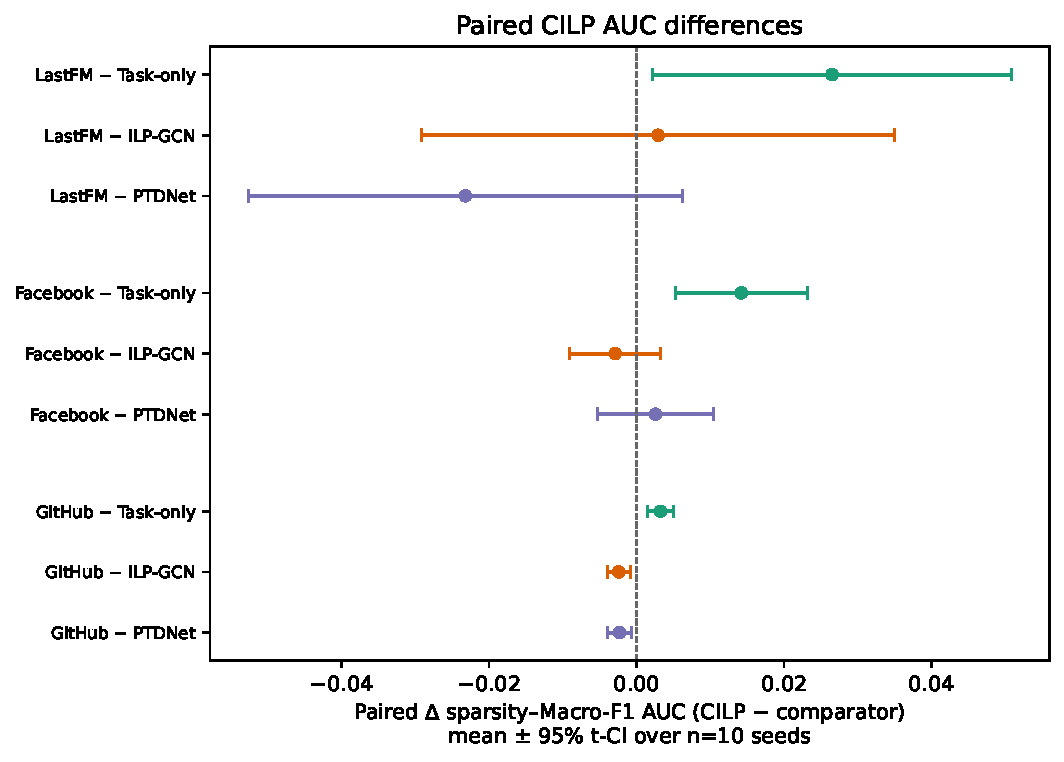
\includegraphics[width=\linewidth]{figures/fig3_method_comparison.pdf}
\caption{\textbf{Paired CILP AUC differences.}
Forest plot of mean CILP$-$comparator sparsity--Macro-F1 AUC with $95\%$ $t$-based CIs ($n{=}10$ seeds).
Positive values favour CILP.}
\label{fig:compare}
\end{figure}

\subsection{Multi-criteria versus task-only counterfactual supervision}
We tested whether combining multiple deletion-importance criteria improves edge ranking relative to task-only supervision under the same encoder, fusion architecture, optimization procedure, removal budgets, and paired seeds.
We considered multi-criteria supervision supported across datasets when it improved at least two seed-aligned evaluation dimensions on at least two datasets under an identical fusion architecture, with Holm adjustment within each dataset's four-metric family~(i) (sparsity--Macro-F1 AUC; giant-component ratio, bridge retention, and minority-degree retention at $50\%$ removal).

On paired seeds $0$--$9$ ($n{=}10$) with concatenation fusion, CILP improves all four metrics over Task-only on LastFM, Facebook, and GitHub (Holm-adjusted Wilcoxon $p{<}0.05$ in family~(i); Supplementary Information~S21; Fig.~\ref{fig:teacher}, Table~\ref{tab:teacher}).
On GitHub the predictive AUC effect is statistically consistent but small in magnitude ($\Delta{=}{+}0.0033$; wins/ties/losses $10/0/0$); statistical significance should not be equated with practical dominance.
The fixed four-metric support criterion is met on all three datasets.
This support is relative to the matched Task-only teacher and does not imply that CILP outperforms all established sparsifiers.

\begin{figure}[t]
\centering
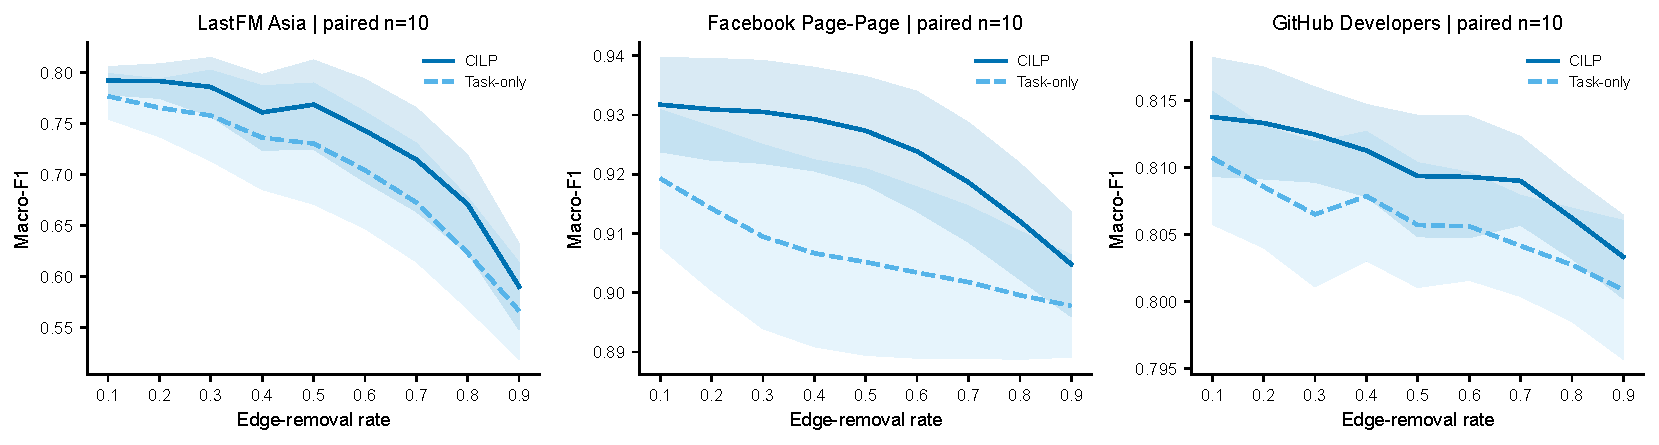
\includegraphics[width=\linewidth]{figures/fig4_teacher_compare.pdf}
\caption{\textbf{Multi-criteria versus task-only supervision.}
Comparison on paired seeds using identical GCN encoders and concatenation fusion ($n{=}10$).
Bands: $t$-based $95\%$ CIs.}
\label{fig:teacher}
\end{figure}

\begin{table}[t]
\centering
\caption{\textbf{Multi-criteria versus task-only counterfactual supervision}
(sparsity--Macro-F1 AUC; paired seeds $0$--$9$).}
\label{tab:teacher}
\scriptsize
\begin{tabular}{@{}lccccccc@{}}
\toprule
Dataset & CILP AUC & Task-only AUC & Paired $\Delta$ & 95\% CI & Wilcoxon $p$ & Holm $p$ & $d_z$ \\
\midrule
LastFM & $0.593{\pm}0.038$ & $0.566{\pm}0.050$ & $+0.0265$ & $[0.0022,0.0508]$ & $0.003906$ & $0.007812$ & $0.781$ \\
Facebook & $0.739{\pm}0.010$ & $0.725{\pm}0.015$ & $+0.0142$ & $[0.0053,0.0231]$ & $0.003906$ & $0.015625$ & $1.137$ \\
GitHub & $0.648{\pm}0.004$ & $0.645{\pm}0.004$ & $+0.0033$ & $[0.0015,0.0051]$ & $0.001953$ & $0.007812$ & $1.292$ \\
\bottomrule
\end{tabular}
\end{table}

\noindent
Win/tie/loss counts for AUC are $9/0/1$ (LastFM), $9/0/1$ (Facebook), and $10/0/0$ (GitHub).

\subsection{Structural and group-preservation results}
At $50\%$ edge removal, CILP preserves connectivity and bridges substantially better than the task-only teacher on all three datasets (Fig.~\ref{fig:structure}, Table~\ref{tab:structure}).
Table~\ref{tab:structure_multi} extends giant-component and bridge retention to $30\%$, $50\%$, and $70\%$ removal so that structural reporting is not restricted to a single operating point.
On GitHub, CILP$-$Task-only differences at $50\%$ are $\Delta_{\mathrm{GC}}{=}{+}0.228$, $\Delta_{\mathrm{bridge}}{=}{+}0.320$, and $\Delta_{\mathrm{mindeg}}{=}{+}0.114$ (Holm $p{=}0.0078$ each in family~(i); W/T/L $=10/0/0$, $10/0/0$, and $9/0/1$).
These structural improvements relative to Task-only are larger than the GitHub predictive AUC gain.
However, CILP is not the overall structural leader: on GitHub, ILP-GCN and PTDNet exceed CILP on giant-component ratio, PTDNet leads minority-degree retention, and CILP leads bridge retention among the reported methods.
On LastFM and Facebook, ILP-GCN likewise remains strong on several structural metrics.
These results support the value of multi-criteria supervision relative to its matched ablation, but not overall structural dominance.
No direct community-preservation metric is currently reported; community enters only as a community-boundary teacher proxy (Supplementary Information~S6).

\begin{figure}[t]
\centering
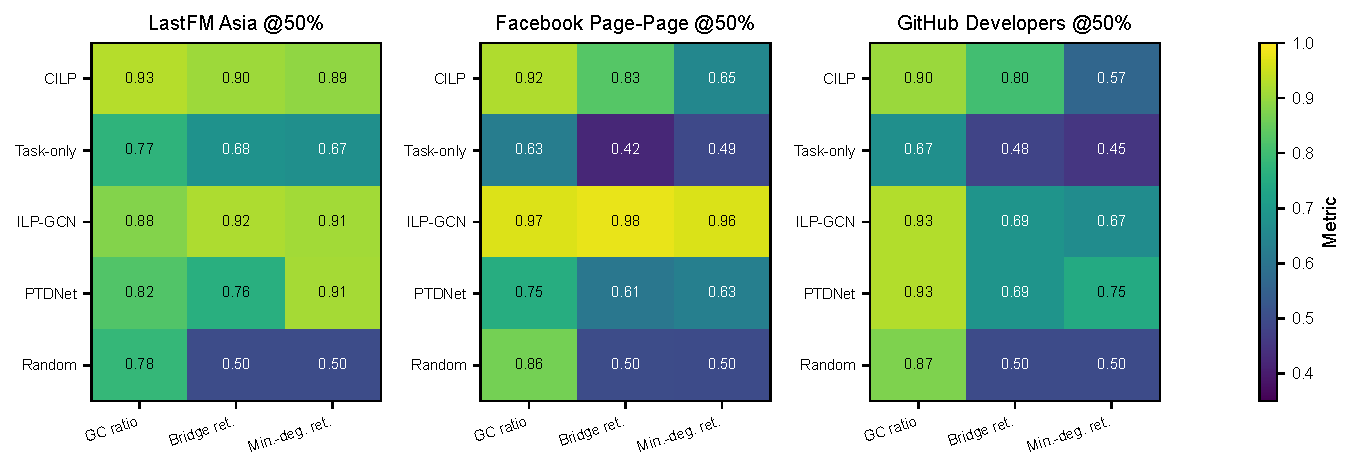
\includegraphics[width=\linewidth]{figures/fig5_structure.pdf}
\caption{\textbf{Structural and group metrics at $50\%$ edge removal} (seed-wise means, $n{=}10$).
Rows denote methods and columns denote metrics.
Cell colours encode metric values using the shared numerical colour scale shown on the right ($[0.35,1.0]$).}
\label{fig:structure}
\end{figure}

\begin{table}[t]
\centering
\caption{\textbf{Structural and group metrics at $50\%$ removal} (means over common seeds).}
\label{tab:structure}
\input{tables/table4_structure.tex}
\end{table}

\begin{table}[t]
\centering
\caption{\textbf{Structural metrics at $30\%$, $50\%$, and $70\%$ removal} (means over $n{=}10$ seeds).
GC: giant-component ratio; Br: bridge retention.}
\label{tab:structure_multi}
\scriptsize
\begin{tabular}{@{}llcccccc@{}}
\toprule
Dataset & Method & GC@30 & GC@50 & GC@70 & Br@30 & Br@50 & Br@70 \\
\midrule
LastFM & CILP & 0.966 & 0.928 & 0.714 & 0.933 & 0.904 & 0.811 \\
LastFM & Task-only & 0.872 & 0.772 & 0.575 & 0.763 & 0.681 & 0.574 \\
LastFM & ILP-GCN & 0.982 & 0.880 & 0.622 & 0.985 & 0.920 & 0.720 \\
LastFM & PTDNet & 0.949 & 0.822 & 0.554 & 0.889 & 0.759 & 0.566 \\
LastFM & Random & 0.894 & 0.784 & 0.602 & 0.700 & 0.501 & 0.300 \\
\midrule
Facebook & CILP & 0.947 & 0.923 & 0.844 & 0.848 & 0.827 & 0.793 \\
Facebook & Task-only & 0.721 & 0.626 & 0.534 & 0.450 & 0.422 & 0.397 \\
Facebook & ILP-GCN & 0.997 & 0.966 & 0.695 & 0.993 & 0.979 & 0.883 \\
Facebook & PTDNet & 0.903 & 0.754 & 0.550 & 0.793 & 0.607 & 0.422 \\
Facebook & Random & 0.937 & 0.863 & 0.731 & 0.703 & 0.502 & 0.300 \\
\midrule
GitHub & CILP & 0.930 & 0.903 & 0.865 & 0.811 & 0.802 & 0.795 \\
GitHub & Task-only & 0.784 & 0.674 & 0.576 & 0.523 & 0.483 & 0.461 \\
GitHub & ILP-GCN & 0.950 & 0.925 & 0.878 & 0.753 & 0.685 & 0.597 \\
GitHub & PTDNet & 0.951 & 0.925 & 0.870 & 0.757 & 0.687 & 0.589 \\
GitHub & Random & 0.941 & 0.873 & 0.750 & 0.700 & 0.500 & 0.299 \\
\bottomrule
\end{tabular}

\end{table}

\subsection{Surrogate quality and uncertainty estimation}
Surrogate--teacher agreement is higher under the multi-criteria teacher than under Task-only on LastFM and Facebook.
On GitHub, CILP attains higher Spearman and Kendall rank agreement, while Task-only has lower raw MAE and ECE is essentially equal (Supplementary Information~S19).
Because pruning ranks edges, rank agreement is the more relevant surrogate diagnostic than absolute regression error; lower MAE alone does not imply a better deletion ranking.
Ranking uses $\mu_e$; $\sigma_e$ is estimated uncertainty and is not an uncertainty-aware pruning rule in reported runs (Supplementary Information~S10).

\subsection{Ablation studies}
LastFM ablations (seeds $0$--$4$; $n{=}5$) are summarized in Fig.~\ref{fig:ablate} by fusion, priors, teacher, and a contextual parent-method comparison.
The Fusion panel holds the multi-criteria teacher fixed and compares concatenation, gated fusion, and cross-attention.
The Teacher panel compares multi-criteria versus task-only under concatenation.
The Context panel contrasts CILP with ILP-GCN and is not a matched ablation.
Leave-one-criterion-out and weight-sensitivity analyses are recommended next steps and are not claimed in the present results.
Adversarial variants were omitted after a negative pilot (Supplementary Information~S20).

\begin{figure}[t]
\centering
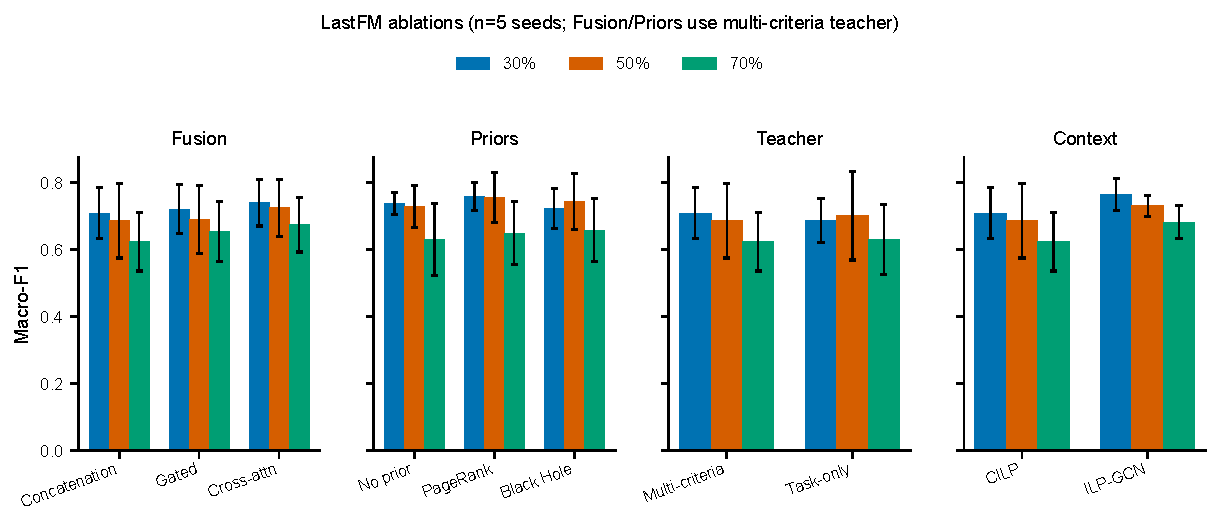
\includegraphics[width=\linewidth]{figures/fig6_ablations.pdf}
\caption{\textbf{LastFM ablations} ($n{=}5$ seeds $0$--$4$).
Fusion and Teacher panels use the multi-criteria teacher unless noted; Context compares CILP with ILP-GCN.
The Priors panel shows a selected subset of three completed prior variants (no prior, PageRank, Black Hole); the full five completed prior variants appear in Supplementary Information~S20.}
\label{fig:ablate}
\end{figure}

\subsection{Runtime}
Wall-clock training times for CILP and Task-only include teacher construction and scorer fitting and were not logged separately (Fig.~\ref{fig:runtime}, Table~\ref{tab:runtime}).
CILP training is therefore substantially more expensive than ILP-GCN and PTDNet on all three datasets, but we do not claim that teacher construction alone dominates that cost.
The full GitHub grid orchestration wall-clock was approximately $6.19$\,h; that figure is an orchestration-level total, not a single method's mean runtime.
Successful completion on GitHub ($37{,}700$ nodes; $289{,}003$ unique undirected edges) demonstrates feasibility at this scale under the reported CPU protocol; it does not establish large-scale GPU efficiency or quantify downstream training speedup after sparsification.

\begin{figure}[t]
\centering
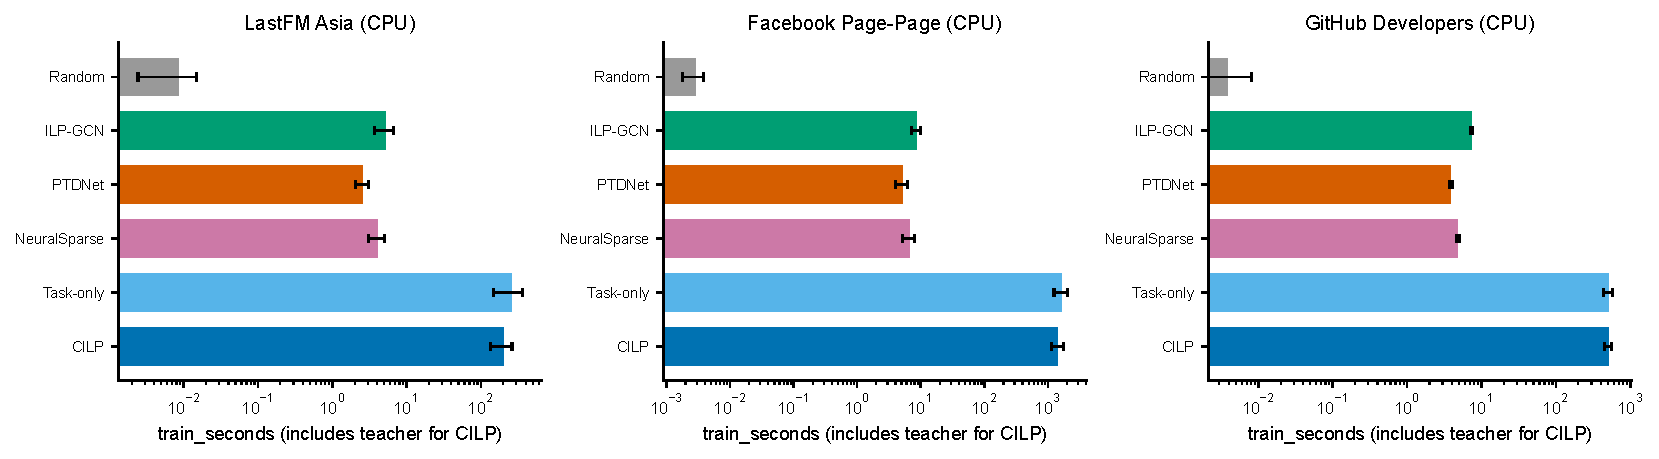
\includegraphics[width=\linewidth]{figures/fig7_runtime.pdf}
\caption{\textbf{Training wall-clock} (CPU, log scale; $n{=}10$).
CILP/Task-only times include the counterfactual teacher.}
\label{fig:runtime}
\end{figure}

\begin{table}[t]
\centering
\caption{\textbf{Runtime} (mean$\pm$s.d.\ training seconds; CPU; $n{=}10$).}
\label{tab:runtime}
\begin{tabular}{@{}lccc@{}}
\toprule
Method & LastFM & Facebook & GitHub \\
\midrule
Random & $0.009{\pm}0.009$ & $0.003{\pm}0.001$ & $0.004{\pm}0.005$ \\
ILP-GCN & $5.2{\pm}2.0$ & $8.6{\pm}2.0$ & $7.4{\pm}0.3$ \\
PTDNet & $2.6{\pm}0.7$ & $5.1{\pm}1.4$ & $3.9{\pm}0.3$ \\
Task-only & $255{\pm}149$ & $1635{\pm}542$ & $504{\pm}94$ \\
CILP & $198{\pm}89$ & $1437{\pm}421$ & $504{\pm}85$ \\
\bottomrule
\end{tabular}
\end{table}

\subsection{Rejected optional hypotheses}
An adversarial variant on LastFM seed~$0$ at $50\%$ removal reached Macro-F1 $\approx0.666$ versus $\approx0.829$ for the core configuration.
A Facebook teacher size of $n{=}40$ underperformed the development-selected $n{=}120$ setting (Supplementary Information~S8).

\section{Discussion}
\label{sec:discussion}

Across three attributed social networks, CILP improves over the architecturally matched task-only teacher under paired seeds and identical fusion, including sparsity--Macro-F1 AUC and the three structural metrics at $50\%$ removal after within-dataset Holm adjustment in family~(i).
The fixed four-metric support criterion is satisfied on LastFM, Facebook, and GitHub.
CILP remains competitive with ILP-GCN and PTDNet for predictive AUC, but it is not universally the predictive leader: PTDNet leads predictive AUC on LastFM, ILP-GCN leads slightly on Facebook, and on GitHub CILP significantly improves over Task-only but remains slightly below ILP-GCN and PTDNet.
On GitHub, the CILP-versus-Task-only AUC improvement is small ($\Delta{=}{+}0.0033$) yet consistent across all ten seeds; structural improvements relative to Task-only are larger than that predictive gain.
ILP-GCN and PTDNet remain strong structural comparators on several metrics, so the contribution is the teacher-based composite supervision framework under matched budgets, not universal predictive or structural leadership.

From a big-data systems perspective, exact-budget pruning is motivated by reduced edge volume for downstream message passing.
The present evidence shows that CILP training---teacher construction plus scorer fitting---is substantially more expensive than ILP-GCN or PTDNet; teacher and scorer times were not separately logged.
Successful completion of the full GitHub grid ($37{,}700$ nodes; $289{,}003$ edges; ten seeds; budgets $0.1$--$0.9$; orchestration wall-clock $\approx6.19$\,h) strengthens feasibility at this scale under the reported protocol; it does not establish industrial-scale GPU efficiency, nor does it yet quantify how many downstream training runs are needed to amortize construction cost.
Separate timers and a downstream break-even analysis are the natural next systems measurements.

Reported pruning is unconstrained ranking by $\mu_e$.
Constraint-aware pruning and $\mu{+}\kappa\sigma$ rules are implemented but unused in the multi-seed comparison.
Community structure enters only as a community-boundary teacher proxy (inter-community edges receive an explicit additive harm term); no direct community-preservation evaluation metric is reported.
For all reported datasets ($|V|{>}400$), the spectral criterion is a degree-based proxy $1/d_u+1/d_v$, not a recomputed Laplacian eigenspectrum difference.
Criterion weights are fixed and untuned; leave-one-criterion-out and weight-sensitivity analyses remain open.
The development partition is reused for teacher $\Delta_{\mathrm{task}}$ and Facebook teacher-size selection, so the protocol is not fully validation-isolated.
Adversarial learning and an under-sized Facebook teacher ($n{=}40$) are retained as rejected pilots.
Limitations therefore include CPU training cost of CILP, the degree-based spectral proxy, fixed $\beta$, development-set reuse, absence of direct community metrics, and a single Resistance proxy rather than independently reproduced classical sparsifiers.
The supported contribution is composite counterfactual supervision under matched budgets relative to a controlled task-only ablation.

\section{Conclusions}
\label{sec:conclusions}

CILP provides a feasible inverse-link-prediction formulation for utility-preserving sparsification of attributed social networks.
Across three attributed social networks---LastFM Asia, Facebook Page-Page, and GitHub Developers---each with ten paired seeds and budgets $0.1$--$0.9$, the multi-criteria teacher consistently improves sparsity--Macro-F1 AUC and structural metrics relative to an architecturally matched task-only teacher under identical fusion and exact budgets.
The fixed four-metric support rule is satisfied on all three datasets.
CILP remains competitive with ILP-GCN and PTDNet on predictive AUC, but it is not universally superior: on GitHub it significantly improves over Task-only yet remains slightly below ILP-GCN and PTDNet.
The supported methodological contribution is therefore composite counterfactual supervision with a controlled ablation, not overall sparsifier leadership.
CILP training, which includes teacher construction and scorer fitting, remains substantially more expensive than lighter baselines.
Future work includes training-only teacher targets, separate teacher/scorer timers, downstream GCN break-even measurement, leave-one-criterion-out and weight-sensitivity analyses, direct community-preservation metrics, full-graph ($0\%$) utility-retention references, adaptive teacher sampling, and validating the spectral proxy.


\section*{List of abbreviations}
\begin{description}[style=nextline,leftmargin=3.2cm,font=\normalfont]
\item[AUC] Area under the sparsity--Macro-F1 curve
\item[CILP] Counterfactual Inverse Link Prediction
\item[GCN] Graph convolutional network
\item[GNN] Graph neural network
\item[ILP-GCN] Inverse link prediction with graph convolutional networks
\item[NLL] Negative log-likelihood
\end{description}

\section*{Declarations}

\subsection*{Ethics approval and consent to participate}
Not applicable.

\subsection*{Consent for publication}
Not applicable.

\subsection*{Availability of data and materials}
Attributed graphs are reconstructed from public SNAP and MUSAE releases~\citep{rozemberczki2021multi} for LastFM Asia, Facebook Page-Page, and GitHub Developers.
Processed graphs, fixed train/development/test splits for seeds $0$--$9$, the authoritative result store ($1{,}890$ rows), per-seed raw outputs, regenerated tables and figures, the Stage~A freeze manifest, the consistency validator, and exact configuration sources accompany the code release.
No DOI is claimed in this draft.

\subsection*{Competing interests}
The authors declare that they have no competing interests.

\subsection*{Funding}
% Finalize funding statement before submission.
Not applicable / to be completed.

\subsection*{Authors' contributions}
% Finalize after authorship is confirmed.
All authors contributed to the conception and design of the study; details to be finalized before submission.

\subsection*{Acknowledgements}
Not applicable / to be completed.

\subsection*{Authors' information}
Optional; to be completed if desired.

\section*{Supplementary information}
Supplementary Information accompanies this article, including teacher definitions, full per-budget tables, paired tests, ablations, hyperparameter and software audits, and runtime logs.

\bibliographystyle{plainnat}
\bibliography{references}

\end{document}
